\documentclass[a0paper,portrait,fleqn,leqno]{tikzposter}
\title{Wegfindung im Labyrinth}
%\institute{Universit\"{a}t Heidelberg}
\author{Florian Nowak \& Yichuan Shen}
%\author{%
%  Florian Nowak\footnote{Florian Nowak: B.\,Sc. Mathematik, 7. Fachsemester}\; \& Yichuan Shen\footnote{Yichuan Shen: M.\,Sc. Mathematik, 1. Fachsemester}\\
%  Betreuer: Gero Plettenberg, Thomas Kloepfer
%  }
\date{Wintersemester 2014/15}

% Für die Bestimmungen aus dem Leitfaden siehe Dokumentende


\settitle{%
  \centering\vbox{%
  \@titlegraphic\\%
  [\TP@titlegraphictotitledistance]\centering\color{titlefgcolor}%
  {\bfseries\Huge\sc\@title\par}%
  \vspace*{1em}%
  {\huge\@author\par}\vspace*{1em}{\LARGE\@date}%
  }}
  
\colorlet{Gray}{black!40}
\colorlet{lightGray}{black!25}
\colorlet{Lime}{lime!50!black!70}
\colorlet{lightLime}{lime!50!black!30}

\definecolorstyle{mystyle}{%
  \definecolor{colorOne}{named}{lightGray}
  \definecolor{colorTwo}{named}{Lime}
  }{%
  % Background Colors
  \colorlet{backgroundcolor}{white}
  \colorlet{framecolor}{colorOne}
  % Title Colors
  \colorlet{titlefgcolor}{black}
  \colorlet{titlebgcolor}{white}
  % Block Colors
  \colorlet{blocktitlebgcolor}{colorTwo}
  \colorlet{blocktitlefgcolor}{white}
  \colorlet{blockbodybgcolor}{white}
  \colorlet{blockbodyfgcolor}{black}
  }

\definelayouttheme{mytheme}{%
  \usecolorstyle{mystyle}
  \usebackgroundstyle{Default} 
  % Predefined Styles: Default, Rays, VerticalGradation, 
  % BottomVerticalGradation, Empty
  \usetitlestyle{Filled} 
  % Default, Basic, Envelope, Wave, VerticalShading, Filled, Empty
  \useblockstyle{Basic}
  % Default, Basic, Minimal, Envelope, Corner, Slide, TornOut
  \useinnerblockstyle{Default} 
  % Default, Table
  \usenotestyle{Sticky} 
  % Default, Corner, VerticalShading, Sticky
  }


\titlegraphic{%
  \includegraphics[scale=2]{unihei_logo_bl}
  }
\usetheme{mytheme}

\usepackage[ngerman]{babel}
\usepackage[utf8]{inputenc}
\usepackage{graphicx,xparse} 

%\usepackage{minted}
%  \usemintedstyle{monokai}
\usepackage{blindtext}


\begin{document}
\maketitle

\block[roundedcorners=0,linewidth=2pt]{Aufgabenstellung}{%
  %\begin{tikzfigure}[Caption]
  %	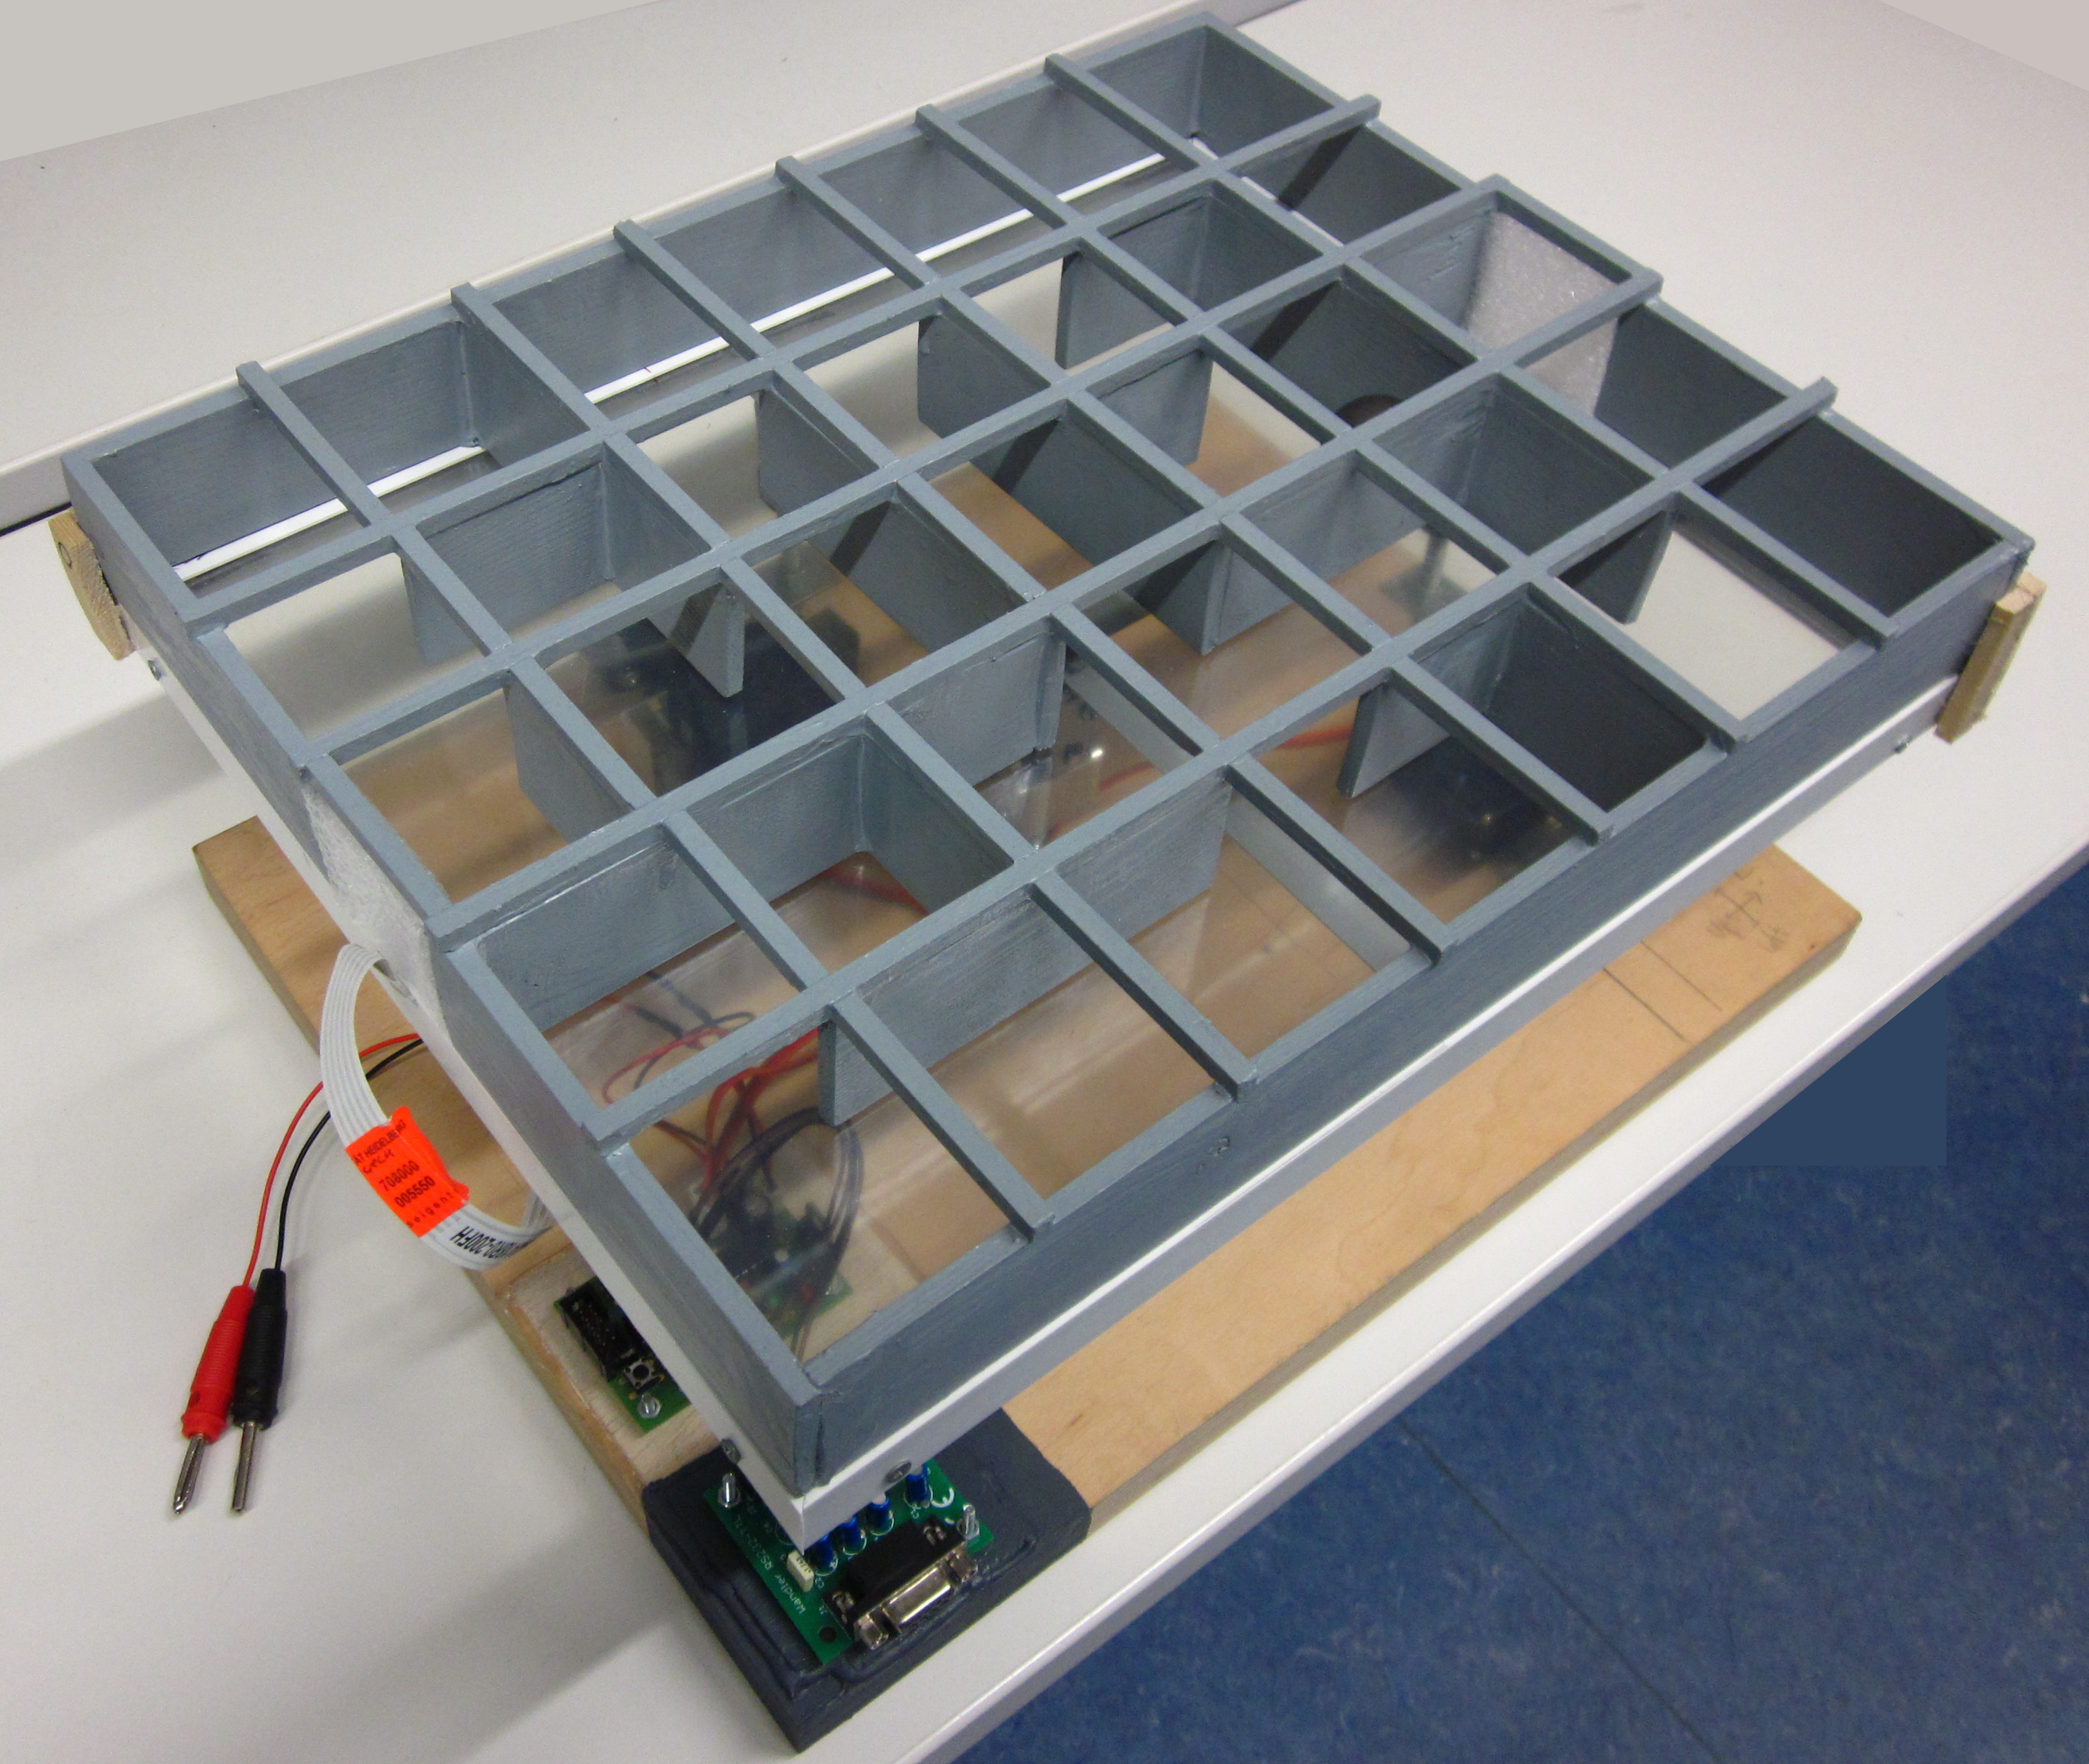
\includegraphics[scale=.5]{roboter_badly-photoshoped}
  %\end{tikzfigure}
  }

\begin{columns}
  \column{.5}
  \block[roundedcorners=0,linewidth=2pt]{Titel}{%
  \blindtext
  \begin{tikzfigure}[Caption of the figure]
  	Figure
  \end{tikzfigure}
  }
  \column{.5}
  \block[roundedcorners=0,linewidth=2pt]{Titel}{Text}
  \block[roundedcorners=0,linewidth=2pt]{Personen}{%
  \textbf{Autoren}\\
  Florian Nowak: B.\,Sc. Mathematik, 7. Fachsemester\\
  Yichuan Shen:\hspace{.1875em} M.\,Sc. Mathematik, 1. Fachsemester
  
  \medskip\noindent
  \textbf{Betreuer}\\
  Gero Plettenberg, Thomas Kloepfer 
  }
\end{columns}

\end{document}

% Auszug aus dem Leitfaden (Abschnitt 7.2):
%
% Das Poster dient dazu, das Ergebnis des Projektes auf eine prägnante und ansprechende Weise darzustellen. Im Gegensatz zur Webpage liegt der Fokus beim Poster auf dem Ergebnis des Praktikums und nicht auf dem Praktikumsverlauf. Das Layout des Posters soll gut strukturiert und optisch ansprechend sein. Zwischen Grafiken und Text soll ein Gleichgewicht herrschen und es soll sichergestellt sein, dass der Betrachter Grafiken dem zugehörigen Text zuordnen kann.
%
% Das Poster beinhaltet folgende Punkte:
% • Titel des Projektes
% • Bearbeitungszeitraum (das jeweilige Semester, in dem das Praktikum absolviert wurde)
% • Name und Studienfächer der Studierenden
% • Betreuer und Supervisor
% • Aufgabenstellung des Projektes
% • Ergebnis
% • Bilder des Roboters, Visualisierung o. Ä.
%
% Das Poster ist in DinA0- oder DinA4- Format als PDF dem jeweiligen Betreuer zu schicken. Auf ausreichende Auflösung der Fotos ist zu achten, außerdem sollten Texte und Graphiken im Vektorformat vorliegen. Die Hintergrundfarbe des Posters ist weiß.